\documentclass[a4paper,12pt]{article}
\usepackage{geometry}
\geometry{a4paper, margin=1in}

\usepackage{amsmath} 
\usepackage{amssymb}
\usepackage{graphicx}
\usepackage{float}
\usepackage[
    colorlinks=true, 
    linkcolor=blue,     
    citecolor=green,    
    urlcolor=blue       
]{hyperref}
\usepackage{booktabs}
\usepackage{caption}
\usepackage[utf8]{inputenc}
\usepackage{subcaption}
\usepackage{tcolorbox}
\usepackage{colortbl}
\usepackage{xcolor}
\usepackage{ragged2e}
\usepackage{algorithm}
\usepackage{algpseudocode}
\usepackage{tikz}
\usetikzlibrary{shapes.geometric, arrows, positioning,shadows}

\bibliographystyle{ieeetr}

\parindent 0px

% Custom Colors
\definecolor{myorange}{rgb}{0.85, 0.49, 0.13}
\definecolor{myblue}{rgb}{0.15, 0.65, 0.90}
\definecolor{mygreen}{rgb}{0.19, 0.82, 0.28}
\definecolor{myred}{rgb}{0.85, 0.11, 0.11}

% ---- Added for Process and Techniques section ----
\usepackage{array}
\usepackage{tabularx}
\usetikzlibrary{arrows.meta, calc, fit, backgrounds}
\definecolor{mypurple}{rgb}{0.55, 0.35, 0.75}

% TikZ styles
\tikzstyle{startstop} = [rectangle, rounded corners, minimum width=3.2cm, minimum height=0.9cm, text centered, draw=black, fill=myred!25, drop shadow]
\tikzstyle{process} = [rectangle, minimum width=3.6cm, minimum height=0.9cm, text centered, text width=3.4cm, draw=black, fill=myblue!25, drop shadow]
\tikzstyle{decision} = [diamond, aspect=2, minimum width=3cm, text centered, text width=2.4cm, draw=black, fill=mygreen!25, drop shadow, inner sep=1pt]
\tikzstyle{io} = [trapezium, trapezium left angle=70, trapezium right angle=110, minimum width=3cm, minimum height=0.9cm, text centered, text width=3cm, draw=black, fill=myorange!25, drop shadow]
\tikzstyle{arrow} = [thick,->,>=stealth]

\newtcolorbox{keybox}[1]{colback=myblue!5, colframe=myblue!70!black, fonttitle=\bfseries, title=#1}

\begin{document}


\begin{titlepage}
    \begin{center}
        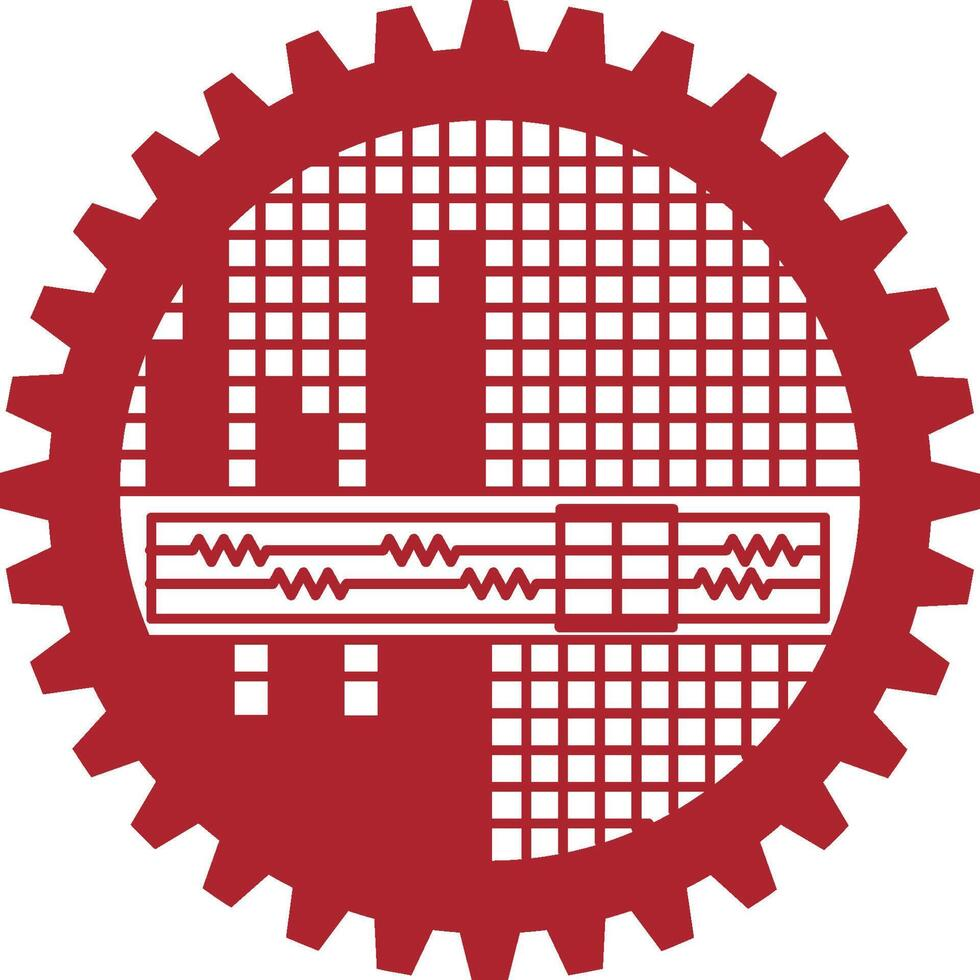
\includegraphics[width=0.25\textwidth]{BUET_logo.jpg} \\
        \vspace{0.5cm}
        \Large{\textbf{CSE200 - Technical Writing and Presentation}} \\
        \vspace{1cm}
        \Large{\textbf{BANGLADESH UNIVERSITY OF ENGINEERING AND TECHNOLOGY}} \\
        \vspace{0.5cm}
        \large{\textbf{DEPARTMENT OF COMPUTER SCIENCE AND ENGINEERING}} \\
        \vspace{2cm}
        \rule{\linewidth}{0.5mm} \\[0.4cm]
        {\Huge{\textbf{Participatory Design Method}}} \\
        \rule{\linewidth}{0.5mm} \\[2cm]
        {\large{\today}} \\[1cm]
        \vfill
        \begin{tabbing}
            \hspace{5cm} \= \hspace{0.5cm} \kill
            Subsection \> : B1 \\ Group \> : 07 \\
            Tajrian Shams Sneha \> : 2305082 \\
            Joyanta Sutradhar \> : 2305083 \\
            Kazi Asef Kabir \> : 2305084 \\
        \end{tabbing}
    \end{center}
\end{titlepage}

\tableofcontents
\listoffigures
\listoftables

\newpage

\begin{center}
    \rule{\linewidth}{0.4mm} \\[1em] % Top line
    \textbf{\Large Participatory Design Method} \\ % Title
    \rule{\linewidth}{0.4mm} % Bottom line
\end{center}

\begin{abstract}
Participatory Design (PD) is a design approach in which the people who will use a system take part in designing it as equal partners, rather than serving only as sources of requirements or test subjects. PD grew out of the Scandinavian workplace democracy movement of the 1970s, which aimed to give workers a real voice in the technologies that shaped their jobs. Since then it has spread to software engineering, human--computer interaction, healthcare, education and public services. In this report we introduce the method and trace its history. We then describe its process, from planning and initial exploration of work through discovery, prototyping and evaluation, together with the key techniques used in each stage, such as contextual inquiry, future workshops, card sorting and cooperative prototyping. We also discuss applications of PD in different domains, its benefits, such as better usability, deeper insight into real work and a stronger sense of ownership, and its challenges, such as conflicting needs, limited time, trust and privacy. We show that, when users hold genuine decision-making power, PD produces systems that fit real work practices and that the people who use them truly own.
\end{abstract}


%==========================================================
\section{Introduction}
\label{sec:introduction}
%==========================================================
Participatory Design (PD) is an approach to designing systems, tools and work environments in which the people who will use them, together with workers, managers and other affected stakeholders, take part as active \textbf{co-designers} rather than serving merely as people whom designers observe, interview or ask to test a finished product~\cite{schuler1993,sanders2008}. This is what separates PD from conventional user-centred design (UCD): in UCD, designers study users and design \emph{for} them, whereas in PD, designers and users design \emph{with} each other, and designers share decision-making power with users instead of holding it alone.

Three ideas underpin this shift. First, PD treats end users as \textbf{design partners}, not as test subjects whose only role is to react to something already built. Second, PD deliberately blends the \textbf{tacit knowledge} that users hold about their own work with the formal expertise of professional designers. Users often find this knowledge difficult to state explicitly but easy to demonstrate. Third, this blending of knowledge forms the conceptual foundation of many present-day \textbf{design patterns} and co-creation methods, from design-thinking workshops to agile story mapping.

\subsection{From User-Centred to Participatory Design}
Table~\ref{tab:ucdvspd} contrasts the two design postures. The essential difference is the direction in which information and authority flow: in UCD it flows one way, from user to designer; in PD it flows both ways, and this reversal shifts the balance of power toward the people who will actually use the system.

\begin{table}[H]
\centering
\begin{tabularx}{\textwidth}{@{}l X X@{}}
\toprule
\rowcolor{myblue!20} \textbf{Aspect} & \textbf{User-Centred Design} & \textbf{Participatory Design} \\
\midrule
Role of the user       & Information source / test subject & Co-designer with a voice in decisions \\
Direction of knowledge & One-way: designer studies user    & Two-way: designer and user learn from each other \\
Decision authority     & Held by the design team           & Shared between designers and participants \\
\bottomrule
\end{tabularx}
\caption{User-Centred Design versus Participatory Design}
\label{tab:ucdvspd}
\end{table}

\subsection{The Collaboration Model}
Meaningful participation depends on bringing together two different kinds of knowledge. Designers contribute \textbf{professional design knowledge}: methods, tools and an understanding of what is technically feasible. Participants contribute \textbf{lived, real-world knowledge}: the practical and contextual understanding of how the work is actually done. Table~\ref{tab:collab} summarizes what each side contributes and what emerges where the two overlap.

\begin{table}[H]
\centering
\begin{tabularx}{\textwidth}{@{}>{\bfseries}l X@{}}
\toprule
\rowcolor{myblue!20} Contributor & Contribution \\
\midrule
Designers    & Professional design knowledge: methods, tools, technical feasibility \\
Participants & Lived, real-world knowledge: work practice, context, everyday constraints \\
Overlap      & Shared understanding, collaboration and capacity-building, supported by common materials (sketches, cards, prototypes) and a shared design environment \\
\bottomrule
\end{tabularx}
\caption{The Participatory Design collaboration model}
\label{tab:collab}
\end{table}

This overlap does not occur in isolation. The wider society and culture in which the project takes place surround and constrain it. They also shape which solutions are acceptable, adoptable and sustainable in practice.

%==========================================================
\section{Historical Background and Evolution}
\label{sec:history}
%==========================================================

\subsection{The Problem Before Participatory Design}
Before PD became established practice, designers and managers created workplace systems and tools in a \textbf{top-down, designer-centric} manner, as Figure~\ref{fig:topdown} illustrates. Decisions flowed in one direction only, from management and designers down to the people who would actually use the resulting system.

\begin{figure}[H]
\centering
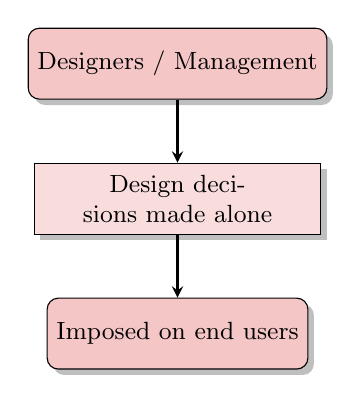
\begin{tikzpicture}[node distance=0.8cm, font=\small]
    \node (a) [startstop] {Designers / Management};
    \node (b) [process, below=of a, fill=myred!15] {Design decisions made alone};
    \node (c) [startstop, below=of b] {Imposed on end users};
    \draw [arrow] (a) -- (b);
    \draw [arrow] (b) -- (c);
\end{tikzpicture}
\caption{The pre-PD, one-way design flow}
\label{fig:topdown}
\end{figure}

Under this model, designers largely ignored users' real needs, context and hard-won workplace expertise. Users could give feedback only \emph{after} launch, when fixing the system was slow, costly or simply impossible. The consequences were predictable: poor usability, low adoption, resistance from the workforce and systems that were technically complete yet solved the \emph{wrong} problem.

\subsection{Origins: The Scandinavian Workplace Democracy Movement}
PD emerged directly as a response to this problem, rooted in the \textbf{Scandinavian workplace democracy movement} of the 1970s~\cite{ehn1988,bansler1989}. Trade unions in Norway, Sweden and Denmark argued that if new computer technology was going to reshape how people worked, the workers affected by that change had a democratic right to help design it, rather than merely giving opinions afterward. Figure~\ref{fig:timeline} traces the resulting evolution of PD from this labour-movement origin to its present form.

\begin{figure}[H]
\centering
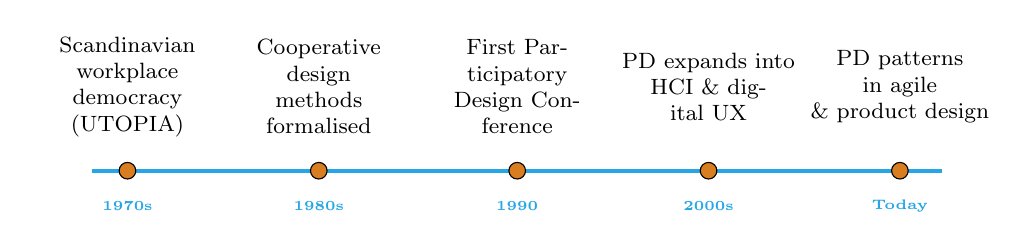
\begin{tikzpicture}[scale=0.9, font=\footnotesize]
    \draw[myblue, line width=1.4pt] (0,0) -- (12,0);
    \foreach \x/\lbl/\yr in {
        0.5/{Scandinavian workplace\\democracy (UTOPIA)}/{1970s},
        3.2/{Cooperative design\\methods formalised}/{1980s},
        6.0/{First Participatory\\Design Conference}/{1990},
        8.7/{PD expands into\\HCI \& digital UX}/{2000s},
        11.4/{PD patterns in agile\\\& product design}/{Today}
      }{
        \node[circle, fill=myorange, draw=black, minimum size=6pt, inner sep=0pt] at (\x,0) {};
        \node[align=center, text width=2.3cm, yshift=6pt] at (\x,0.95) {\lbl};
        \node[font=\bfseries\tiny, myblue] at (\x,-0.5) {\yr};
      }
\end{tikzpicture}
\caption{Timeline of Participatory Design from its Scandinavian origins to today}
\label{fig:timeline}
\end{figure}

\begin{keybox}{Key Milestone}
The \textbf{UTOPIA project} (Scandinavia, late 1970s--80s) brought Nordic trade unions together with researchers to let \emph{typesetters}, whose jobs were directly threatened by new computer typesetting systems, co-design their own tools. Many researchers regard it as the origin of Participatory Design~\cite{ehn1988}.
\end{keybox}

\subsection{How Participatory Design Solved It}
Figure~\ref{fig:beforeafter} contrasts the pre-PD flow with the participatory alternative it gave rise to.

\begin{figure}[H]
\centering
\begin{subfigure}{0.47\textwidth}
\centering
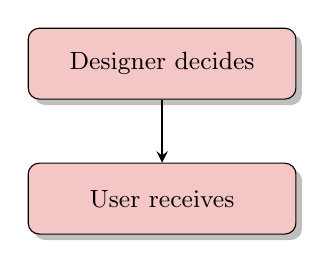
\begin{tikzpicture}[node distance=0.8cm, font=\small]
    \node (d1) [startstop, minimum width=3.4cm] {Designer decides};
    \node (d2) [startstop, below=of d1, minimum width=3.4cm] {User receives};
    \draw [arrow] (d1) -- (d2);
\end{tikzpicture}
\caption{Before: top-down}
\end{subfigure}
\hfill
\begin{subfigure}{0.47\textwidth}
\centering
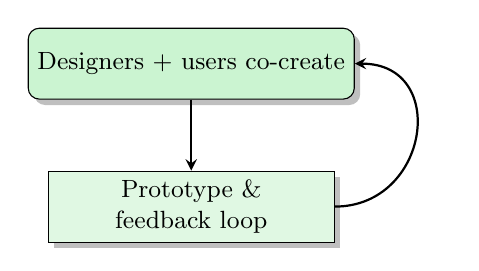
\begin{tikzpicture}[node distance=0.9cm, font=\small]
    \node (p1) [startstop, fill=mygreen!25, minimum width=3.6cm] {Designers + users co-create};
    \node (p2) [process, below=of p1, fill=mygreen!15, minimum width=3.6cm] {Prototype \& feedback loop};
    \draw [arrow] (p1) -- (p2);
    \draw [arrow] (p2.east) .. controls +(1.2,0) and +(1.2,0) .. (p1.east);
\end{tikzpicture}
\caption{After: participatory}
\end{subfigure}
\caption{From a one-way handoff to a cyclical, co-owned process}
\label{fig:beforeafter}
\end{figure}

Empowerment replaced imposition: stakeholders gained a genuine voice and real decision-making power, and design became an \textbf{iterative, cyclical conversation} between designers and users rather than a one-time handoff from one side to the other.

%==========================================================
\section{Core Principles of Participatory Design}
\label{sec:principles}
%==========================================================
The historical shift described above rests on four core principles that recur throughout every stage of the PD process described in the remainder of this report. Table~\ref{tab:principles} summarizes them.

\begin{table}[H]
\centering
\begin{tabularx}{\textwidth}{@{}>{\bfseries}l X@{}}
\toprule
\rowcolor{myblue!20} Principle & Description \\
\midrule
Mutual Learning & Designers learn the domain from users, while users learn design thinking from designers; knowledge flows in both directions and builds a shared understanding. \\
Co-creation \& Ownership & Designers build the system together with its future users, so that it feels like theirs; shared ownership leads to stronger buy-in and better long-term outcomes. \\
Iterative Prototyping & Design proceeds through small, testable steps rather than one big launch; rapid build--test--refine cycles keep the design grounded in real practice. \\
Democratic Decision-Making & No single voice, whether manager, designer or senior user, controls the outcome; every stakeholder holds an equal seat at the table. \\
\bottomrule
\end{tabularx}
\caption{Core principles of Participatory Design}
\label{tab:principles}
\end{table}

These four principles are not independent add-ons; they reinforce one another. Democratic decision-making only functions once mutual learning has given every participant enough shared understanding to make an informed choice, and iterative prototyping is what turns co-creation from a one-off workshop into genuine, lasting ownership of the final system. The remainder of this report describes the concrete process and techniques through which PD teams put these principles into practice.

%==========================================================
\section{The Participatory Design Process}
%==========================================================
We describe PD as a structured yet iterative process in which
designers, developers and end users act as \textbf{co-designers}~\cite{schuler1993,sanders2008}. Following the widely
used three-stage framework of Spinuzzi~\cite{spinuzzi2005}, we divide the process into the following stages:

\begin{enumerate}
    \item \textbf{Initial Exploration of Work:} Designers meet the users, observe how people currently work and understand the tools, workflows, routines and social context.
    \item \textbf{Discovery Processes:} Designers and users collaboratively clarify goals, values and the desired outcome of the system, using workshops, storytelling and organizing techniques.
    \item \textbf{Prototyping:} Users and designers iteratively shape technological artifacts (paper mock-ups, low- and high-fidelity prototypes) until the design fits the envisioned work practice.
\end{enumerate}

Before and after these three core stages, practical projects also include a \textbf{planning} stage (stakeholder identification, recruitment) and an \textbf{evaluation \& deployment} stage. Figure~\ref{fig:cycle} shows the complete cycle.

\begin{figure}[H]
\centering
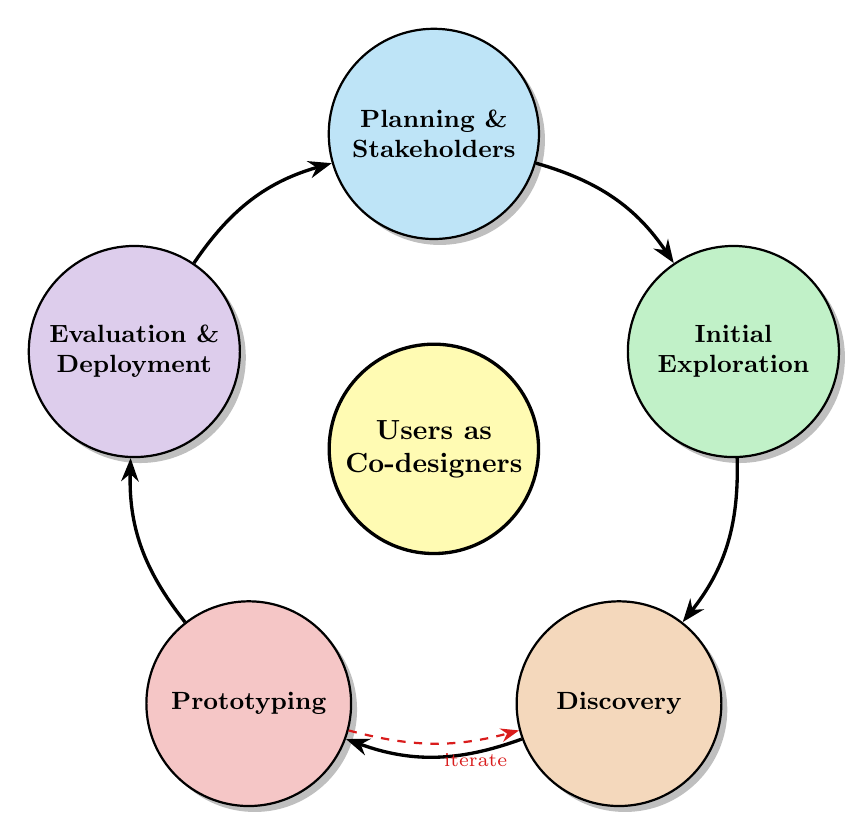
\begin{tikzpicture}[
    node distance=1cm,
    stage/.style={circle, draw=black, thick, minimum size=2.6cm, text width=2.3cm, align=center, font=\small\bfseries, drop shadow}]
    \node[stage, fill=myblue!30]   (a) at (90:4)  {Planning \& Stakeholders};
    \node[stage, fill=mygreen!30]  (b) at (18:4)  {Initial Exploration};
    \node[stage, fill=myorange!30] (c) at (-54:4) {Discovery};
    \node[stage, fill=myred!25]    (d) at (-126:4){Prototyping};
    \node[stage, fill=mypurple!30] (e) at (162:4) {Evaluation \& Deployment};
    \node[circle, draw, very thick, fill=yellow!30, minimum size=2.4cm, align=center, font=\bfseries] at (0,0) {Users as\\Co-designers};
    \draw[->, >=Stealth, very thick, bend left=20] (a) to (b);
    \draw[->, >=Stealth, very thick, bend left=20] (b) to (c);
    \draw[->, >=Stealth, very thick, bend left=20] (c) to (d);
    \draw[->, >=Stealth, very thick, bend left=20] (d) to (e);
    \draw[->, >=Stealth, very thick, bend left=20] (e) to (a);
    \draw[->, >=Stealth, thick, dashed, myred] (d) to[bend right=15] node[midway, below right, font=\scriptsize]{iterate} (c);
\end{tikzpicture}
\caption{The iterative Participatory Design cycle}
\label{fig:cycle}
\end{figure}

\subsection{Simple Model of Iteration}
Each iteration improves the design using the feedback of all participants. If $D_k$ is the design after iteration $k$ and $f_u$ is the feedback of participant $u$ among $N$ participants, then
\begin{equation}
    D_{k+1} = D_k + \frac{1}{N}\sum_{u=1}^{N} f_u(D_k)
\end{equation}
Every participant gets an equal voice, $w_u = 1/N$, which reflects the democratic nature of PD.

\subsection{Overall Process Flowchart}
Figure~\ref{fig:flow} shows the complete process as a flowchart, including the loops back to prototyping and discovery.
\begin{figure}[H]
\centering
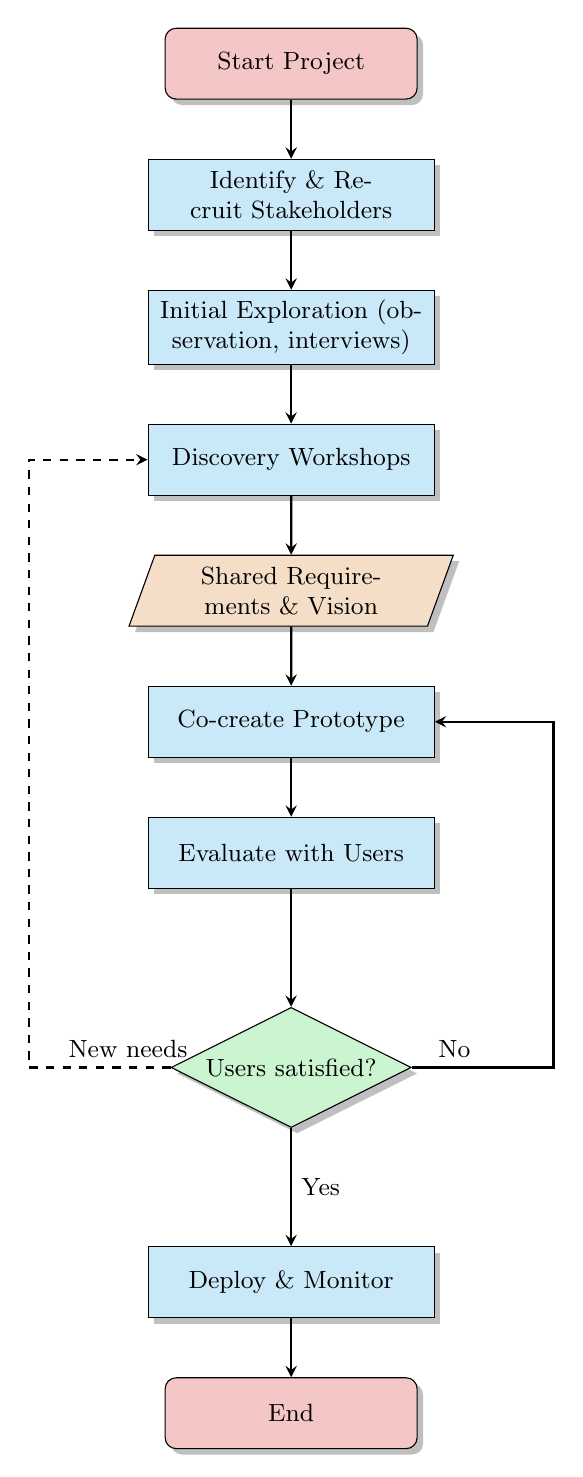
\begin{tikzpicture}[node distance=0.75cm, font=\small]
    \node (start) [startstop] {Start Project};
    \node (stake) [process, below=of start] {Identify \& Recruit Stakeholders};
    \node (explore) [process, below=of stake] {Initial Exploration (observation, interviews)};
    \node (disc) [process, below=of explore] {Discovery Workshops};
    \node (req) [io, below=of disc] {Shared Requirements \& Vision};
    \node (proto) [process, below=of req] {Co-create Prototype};
    \node (eval) [process, below=of proto] {Evaluate with Users};
    \node (dec) [decision, below=1.5cm of eval] {Users satisfied?};
    \node (deploy) [process, below=1.5cm of dec] {Deploy \& Monitor};
    \node (stop) [startstop, below=of deploy] {End};

    \draw [arrow] (start) -- (stake);
    \draw [arrow] (stake) -- (explore);
    \draw [arrow] (explore) -- (disc);
    \draw [arrow] (disc) -- (req);
    \draw [arrow] (req) -- (proto);
    \draw [arrow] (proto) -- (eval);
    \draw [arrow] (eval) -- (dec);
    \draw [arrow] (dec) -- node[right] {Yes} (deploy);
    \draw [arrow] (deploy) -- (stop);
    \draw [arrow] (dec.east) -- ++(1.8,0) node[above, pos=0.3] {No} |- (proto.east);
    \draw [arrow, dashed] (dec.west) -- ++(-1.8,0) node[above, pos=0.3] {New needs} |- (disc.west);
\end{tikzpicture}
\caption{Flowchart of the complete Participatory Design process}
\label{fig:flow}
\end{figure}

%==========================================================
\section{Stage 0: Planning and Stakeholder Identification}
%==========================================================
Participation is only meaningful when the \emph{right} people participate. The planning stage identifies every group that will use the system, feel its effects or influence it.

Designers usually map stakeholders by their \textbf{power} and \textbf{interest}~\cite{eden1998}. PD gives special attention to end users who are strongly affected by the system but have little power, so that their voice is not lost. Figure~\ref{fig:grid} shows the power--interest grid that we use to plan participation.

\subsection{Power--Interest Grid}
\begin{figure}[H]
\centering
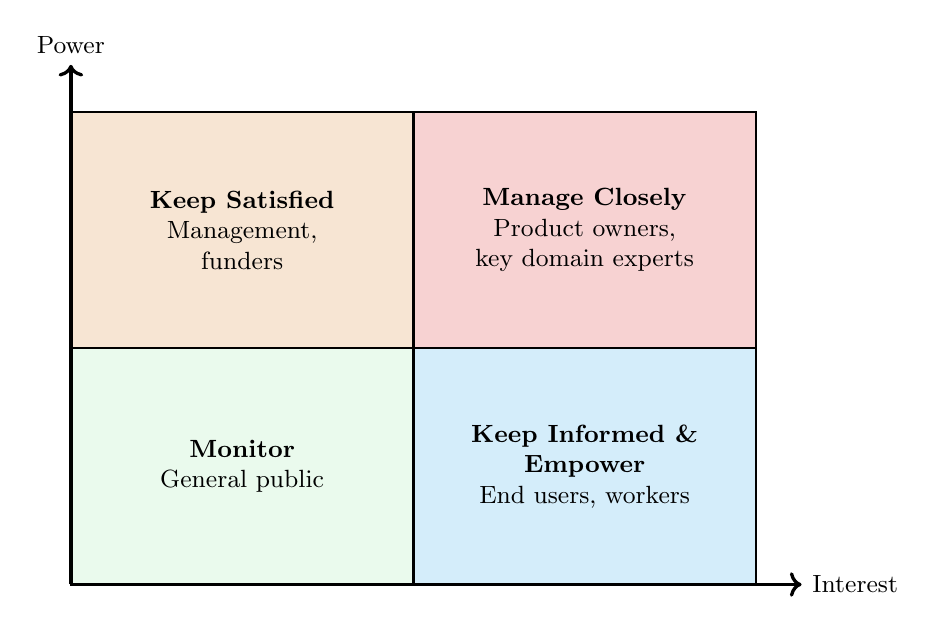
\begin{tikzpicture}[xscale=1.45, every node/.style={font=\small}]
    \fill[myorange!20] (0,3) rectangle (3,6);
    \fill[myred!20] (3,3) rectangle (6,6);
    \fill[mygreen!10] (0,0) rectangle (3,3);
    \fill[myblue!20] (3,0) rectangle (6,3);
    \draw[thick] (0,0) rectangle (6,6);
    \draw[thick] (3,0) -- (3,6); \draw[thick] (0,3) -- (6,3);
    \draw[->, very thick] (0,0) -- (6.4,0) node[right] {Interest};
    \draw[->, very thick] (0,0) -- (0,6.6) node[above] {Power};
    \node[align=center] at (1.5,4.5) {\textbf{Keep Satisfied}\\ \small Management,\\ \small funders};
    \node[align=center] at (4.5,4.5) {\textbf{Manage Closely}\\ \small Product owners,\\ \small key domain experts};
    \node[align=center] at (1.5,1.5) {\textbf{Monitor}\\ \small General public};
    \node[align=center] at (4.5,1.5) {\textbf{Keep Informed \&}\\ \textbf{Empower}\\ \small End users, workers};
\end{tikzpicture}
\caption{Power--Interest grid used to plan participation}
\label{fig:grid}
\end{figure}

\subsection{Levels of Participation}
Not every project gives users the same influence. The project team uses Arnstein's \emph{Ladder of Participation}~\cite{arnstein1969} to decide the intended level before the project starts. Figure~\ref{fig:ladder} shows the eight rungs of the ladder, grouped into non-participation, tokenism and real power.

\begin{figure}[H]
\centering
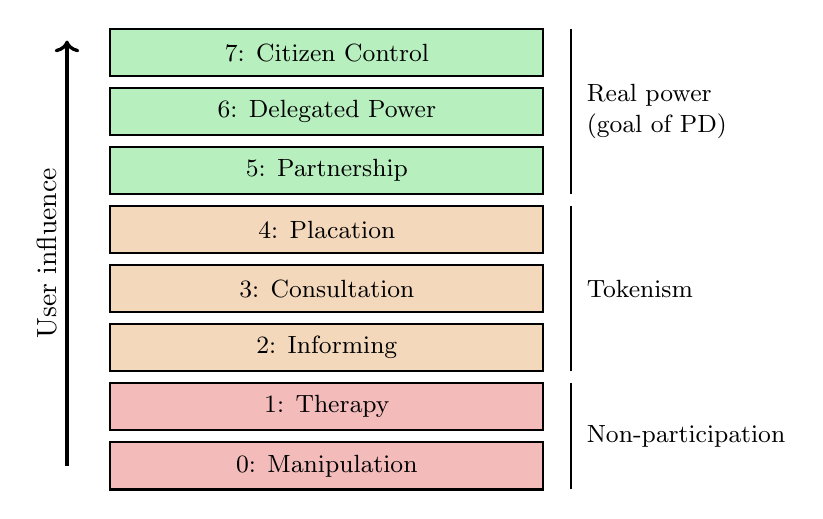
\begin{tikzpicture}[rung/.style={draw, thick, minimum width=5.5cm, minimum height=0.6cm, font=\small}]
    \foreach \y/\t/\c in {0/Manipulation/myred!30, 1/Therapy/myred!30, 2/Informing/myorange!30, 3/Consultation/myorange!30, 4/Placation/myorange!30, 5/Partnership/mygreen!35, 6/Delegated Power/mygreen!35, 7/Citizen Control/mygreen!35}
        \node[rung, fill=\c] at (0,\y*0.75) {\y: \t};
    \draw[thick] (3.1,-0.3) -- (3.1,1.05) node[midway, right=2pt, font=\small] {Non-participation};
    \draw[thick] (3.1,1.2) -- (3.1,3.3) node[midway, right=2pt, font=\small] {Tokenism};
    \draw[thick] (3.1,3.45) -- (3.1,5.55) node[midway, right=2pt, font=\small, align=left] {Real power\\(goal of PD)};
    \draw[->, very thick] (-3.3,0) -- (-3.3,5.4) node[midway, left, rotate=90, anchor=south] {User influence};
\end{tikzpicture}
\caption{Ladder of participation; genuine PD targets the upper rungs}
\label{fig:ladder}
\end{figure}

%==========================================================
\section{Stage 1: Initial Exploration of Work}
%==========================================================
In this stage designers enter the users' world. The goal is to understand \emph{tacit knowledge}: the skills and routines users apply without being able to easily describe them.

\subsection{Techniques}
\begin{itemize}
    \item \textbf{Ethnographic Observation:} Designers observe users in their natural working environment over days or weeks.
    \item \textbf{Contextual Inquiry:} A master--apprentice style interview while the user performs real tasks; the designer asks ``why'' at every step~\cite{beyer1998}.
    \item \textbf{Walkthroughs:} Users walk designers through a typical day or process, explaining each artifact they use.
    \item \textbf{Artifact Analysis:} Designers collect and study the forms, notes, spreadsheets and ``workarounds'' that users create.
    \item \textbf{Semi-structured Interviews:} Flexible interviews guided by open-ended questions.
\end{itemize}

\subsection{How Many Sessions?}
Exploration continues until new sessions stop revealing new themes. If $T_n$ is the number of themes found after $n$ sessions, the share of new themes is
\begin{equation}
    \rho_n = \frac{T_n - T_{n-1}}{T_{n-1}}
\end{equation}
and exploration can stop when $\rho_n$ becomes very small (e.g.\ below $5\%$). In practice, small repeated sessions with around five users each already uncover most of the important problems~\cite{nielsen1993,guest2006}.

%==========================================================
\section{Stage 2: Discovery Processes}
%==========================================================
The discovery stage brings designers and users together to \emph{interpret} what they observed and to envision the future. Its outputs are shared goals, prioritized requirements and a common language.

\subsection{Discovery Techniques}
\begin{itemize}
    \item \textbf{Future Workshop:} A three-phase workshop (Critique $\rightarrow$ Fantasy $\rightarrow$ Implementation) that moves from problems to utopian ideas to realistic plans~\cite{jungk1987}.
    \item \textbf{Card Sorting:} Participants group cards containing features or concepts into categories that make sense to them, revealing their mental model~\cite{spencer2009}.
    \item \textbf{Affinity Diagramming:} Participants write observations on sticky notes and cluster them by similarity to reveal themes.
    \item \textbf{Storytelling and Scenarios:} Users narrate real incidents; these become scenarios and personas.
    \item \textbf{Organizational Games:} Role-play of workflows using cards and boards to explore alternatives.
    \item \textbf{Design Games (e.g.\ CARD, Layout Kit):} Game-like tools that let non-technical users express design ideas.
    \item \textbf{Mock-ups and Collages:} Users create visual collages expressing feelings and expectations.
\end{itemize}

\subsection{Future Workshop Structure}
Figure~\ref{fig:future} shows the four phases of a Future Workshop.
\begin{figure}[H]
\centering
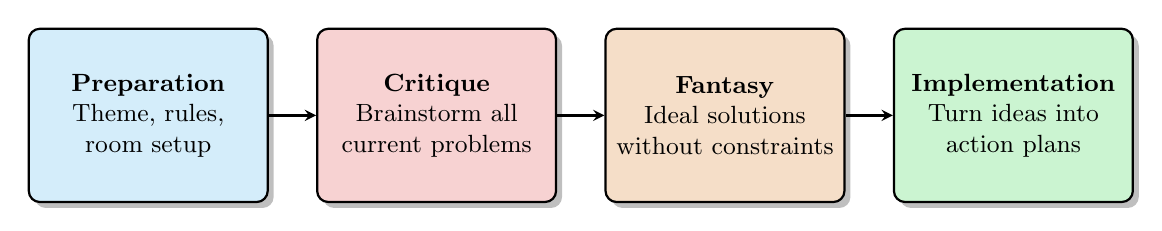
\begin{tikzpicture}[node distance=0.6cm, box/.style={draw, thick, rounded corners, minimum height=2.2cm, text width=2.8cm, align=center, font=\small, drop shadow}]
    \node[box, fill=myblue!20] (p) {\textbf{Preparation}\\ Theme, rules, room setup};
    \node[box, fill=myred!20, right=of p] (c) {\textbf{Critique}\\ Brainstorm all current problems};
    \node[box, fill=myorange!25, right=of c] (f) {\textbf{Fantasy}\\ Ideal solutions without constraints};
    \node[box, fill=mygreen!25, right=of f] (i) {\textbf{Implementation}\\ Turn ideas into action plans};
    \draw[arrow] (p) -- (c); \draw[arrow] (c) -- (f); \draw[arrow] (f) -- (i);
\end{tikzpicture}
\caption{The phases of a Future Workshop}
\label{fig:future}
\end{figure}

\subsection{Card Sorting Analysis}
Suppose $N$ participants sort $m$ cards. For each pair of cards $(i,j)$ let $n_{ij}$ be the number of participants who placed both cards in the same group. The \textbf{similarity matrix} is
\begin{equation}
    S_{ij} = \frac{n_{ij}}{N}, \qquad 0 \le S_{ij} \le 1, \qquad S_{ii} = 1
\end{equation}
and the corresponding distance matrix is $d_{ij} = 1 - S_{ij}$. For example, with four cards and $N=10$ participants:
\begin{equation}
    S = \begin{bmatrix}
        1.0 & 0.8 & 0.1 & 0.2 \\
        0.8 & 1.0 & 0.2 & 0.1 \\
        0.1 & 0.2 & 1.0 & 0.9 \\
        0.2 & 0.1 & 0.9 & 1.0
    \end{bmatrix}
\end{equation}
Cards 1--2 and 3--4 clearly form two groups. We merge cards with high similarity step by step, as Algorithm~\ref{alg:cluster} describes, and Figure~\ref{fig:dendro} shows the resulting dendrogram.

\begin{algorithm}[H]
\caption{Hierarchical Clustering of Card Sort Data}
\label{alg:cluster}
\begin{algorithmic}[1]
\Require Card sorts from $N$ participants, $m$ cards, cut threshold $\tau$
\State Compute $n_{ij}$ for all pairs; set $S_{ij} \gets n_{ij}/N$, $d_{ij} \gets 1 - S_{ij}$
\State Initialize clusters $C \gets \{\{1\},\{2\},\dots,\{m\}\}$
\While{$|C| > 1$}
    \State Find $(A,B) = \arg\min_{A \ne B \in C} d(A,B)$
    \If{$d(A,B) > \tau$}
        \State \textbf{break} \Comment{remaining groups are too dissimilar}
    \EndIf
    \State $C \gets (C \setminus \{A,B\}) \cup \{A \cup B\}$
    \State Record merge $(A,B,d(A,B))$ in dendrogram
\EndWhile
\State \Return $C$ as the categories of the information architecture
\end{algorithmic}
\end{algorithm}

\begin{figure}[H]
\centering
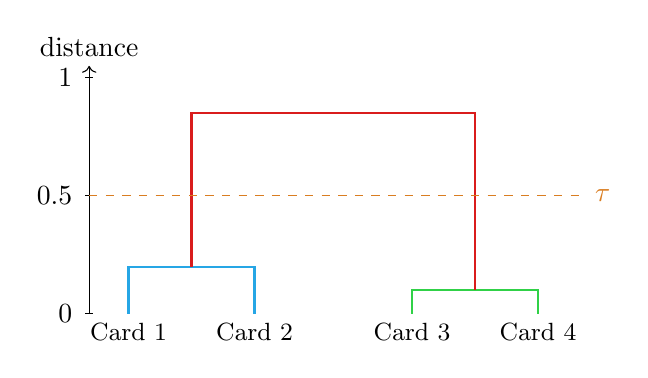
\begin{tikzpicture}[yscale=3]
    \draw[->] (-0.5,0) -- (-0.5,1.05) node[above] {distance};
    \foreach \y in {0,0.5,1} \draw (-0.55,\y) -- (-0.45,\y) node[left=4pt] {\y};
    \foreach \x/\l in {0/Card 1,1.6/Card 2,3.6/Card 3,5.2/Card 4} \node[below] at (\x,0) {\small \l};
    \draw[thick, myblue] (0,0) -- (0,0.2) -- (1.6,0.2) -- (1.6,0);
    \draw[thick, mygreen] (3.6,0) -- (3.6,0.1) -- (5.2,0.1) -- (5.2,0);
    \draw[thick, myred] (0.8,0.2) -- (0.8,0.85) -- (4.4,0.85) -- (4.4,0.1);
    \draw[dashed, myorange] (-0.5,0.5) -- (5.8,0.5) node[right] {$\tau$};
\end{tikzpicture}
\caption{Dendrogram of the example card sort; cutting at $\tau$ gives two categories}
\label{fig:dendro}
\end{figure}

\subsection{Affinity Diagramming}
Figure~\ref{fig:affinity} shows an example affinity diagram, in which raw observations form three themes.
\begin{figure}[H]
\centering
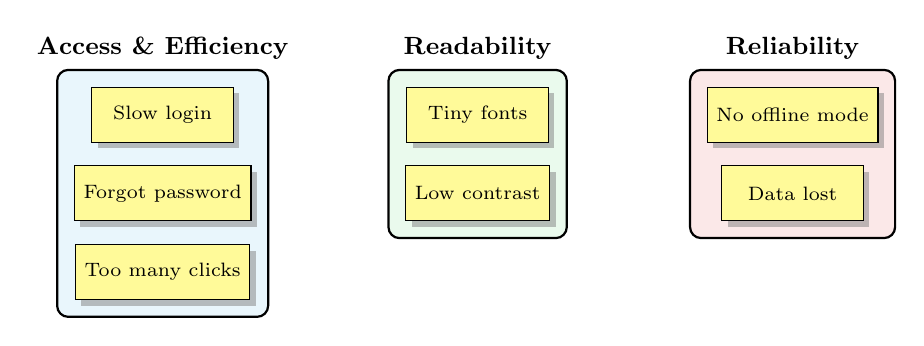
\begin{tikzpicture}[note/.style={draw, fill=yellow!40, minimum width=1.8cm, minimum height=0.7cm, font=\scriptsize, drop shadow}, grp/.style={draw, thick, rounded corners, inner sep=6pt}]
    \node[note] (n1) at (0,0) {Slow login};
    \node[note] (n2) at (0,-1) {Forgot password};
    \node[note] (n3) at (0,-2) {Too many clicks};
    \node[note] (n4) at (4,0) {Tiny fonts};
    \node[note] (n5) at (4,-1) {Low contrast};
    \node[note] (n6) at (8,0) {No offline mode};
    \node[note] (n7) at (8,-1) {Data lost};
    \begin{scope}[on background layer]
    \node[grp, fill=myblue!10, fit=(n1)(n2)(n3), label=above:{\small\bfseries Access \& Efficiency}] {};
    \node[grp, fill=mygreen!10, fit=(n4)(n5), label=above:{\small\bfseries Readability}] {};
    \node[grp, fill=myred!10, fit=(n6)(n7), label=above:{\small\bfseries Reliability}] {};
    \end{scope}
\end{tikzpicture}
\caption{Affinity diagram: raw observations clustered into themes}
\label{fig:affinity}
\end{figure}

\subsection{Collaborative Prioritization}
After collecting ideas, participants prioritize them together, most commonly by dot voting. Table~\ref{tab:vote} shows an example outcome.

\paragraph{Dot Voting.} Each participant $u$ receives $k$ dots to distribute among $m$ ideas. The score of idea $j$ is
\begin{equation}
    V_j = \sum_{u=1}^{N} v_{uj}, \qquad \sum_{j=1}^{m} v_{uj} = k
\end{equation}
where $v_{uj}$ is the number of dots that participant $u$ gives to idea $j$.

\begin{table}[H]
\centering
\begin{tabular}{@{}lcc@{}}
\toprule
\rowcolor{myblue!20} \textbf{Idea} & \textbf{Dot votes $V_j$} & \textbf{Final Rank} \\
\midrule
Offline mode      & 14 & 1 \\
Larger font option & 11 & 2 \\
One-click login   & 9  & 3 \\
Dark theme        & 4  & 4 \\
\bottomrule
\end{tabular}
\caption{Example prioritization outcome of a discovery workshop }
\label{tab:vote}
\end{table}

%==========================================================
\section{Stage 3: Prototyping}
%==========================================================
In the prototyping stage, the shared vision becomes tangible. Users do not only comment on prototypes; they \textbf{build and modify} them.

\subsection{Prototyping Techniques}
\begin{itemize}
    \item \textbf{Paper Prototyping:} Designers draw screens on paper; one person ``plays computer'' while users interact.
    \item \textbf{PICTIVE} (Plastic Interface for Collaborative Technology Initiatives through Video Exploration): Users and developers arrange paper and plastic interface elements on a shared table while a camera records the session~\cite{muller1991}.
    \item \textbf{Cooperative Prototyping:} Designers change a software prototype live while users test it~\cite{bodker1991}.
    \item \textbf{Wizard of Oz:} A hidden human simulates system intelligence, allowing users to test concepts that are not yet built~\cite{kelley1984}.
    \item \textbf{Mock-ups and Role-play:} Physical models of devices or work spaces used in realistic scenarios.
    \item \textbf{Low- to High-fidelity progression:} Sketches $\rightarrow$ wireframes $\rightarrow$ clickable prototypes $\rightarrow$ functional systems.
\end{itemize}

\subsection{Fidelity versus Cost}
Changing a high-fidelity prototype is far more expensive than changing a paper sketch. Therefore PD starts with cheap, low-fidelity materials and raises fidelity only as the design becomes stable.

\subsection{Iterative Prototyping Loop}
Figure~\ref{fig:protoloop} shows the iterative prototyping loop, and Algorithm~\ref{alg:proto} describes one cooperative prototyping session in detail. Both use the System Usability Scale (SUS) score, a usability rating from zero to 100 that Section~\ref{sec:eval} explains.
\begin{figure}[H]
\centering
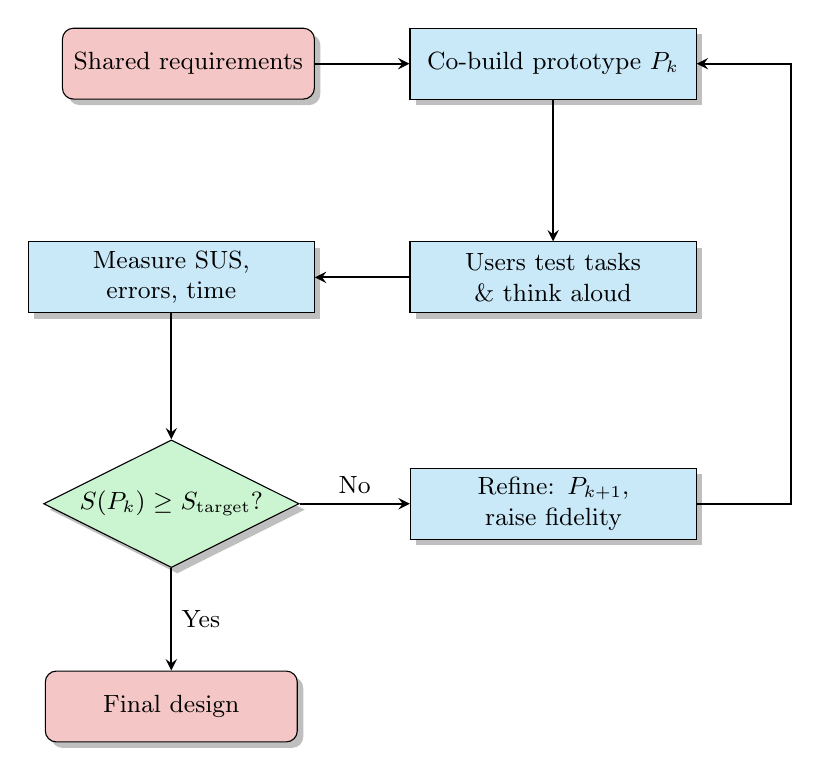
\begin{tikzpicture}[node distance=1.8cm, font=\small]
    \node (s) [startstop] {Shared requirements};
    \node (b) [process, right=1.2cm of s] {Co-build prototype $P_k$};
    \node (t) [process, below=of b] {Users test tasks \& think aloud};
    \node (m) [process, left=1.2cm of t] {Measure SUS, errors, time};
    \node (d) [decision, below=1.6cm of m] {$S(P_k) \ge S_{\text{target}}$?};
    \node (r) [process, right=1.4cm of d] {Refine: $P_{k+1}$, raise fidelity};
    \node (e) [startstop, below=1.3cm of d] {Final design};
    \draw[arrow] (s) -- (b);
    \draw[arrow] (b) -- (t);
    \draw[arrow] (t) -- (m);
    \draw[arrow] (m) -- (d);
    \draw[arrow] (d) -- node[above] {No} (r);
    \draw[arrow] (r) -| ($(b.east)+(1.2,0)$) -- (b.east);
    \draw[arrow] (d) -- node[right] {Yes} (e);
\end{tikzpicture}
\caption{Iterative cooperative prototyping loop}
\label{fig:protoloop}
\end{figure}

\begin{algorithm}[H]
\caption{Cooperative Prototyping Session}
\label{alg:proto}
\begin{algorithmic}[1]
\Require Requirements $R$, participants $U$, target score $S_{\text{target}}$, max iterations $K$
\State $P_0 \gets$ low-fidelity paper prototype from $R$; $k \gets 0$
\Repeat
    \ForAll{$u \in U$}
        \State $u$ performs scenario tasks on $P_k$ while thinking aloud
        \State Record issues $I_u$, task time $t_u$, success $s_u$, SUS score $\text{SUS}_u$
        \State $u$ physically modifies $P_k$ to show preferred solution
    \EndFor
    \State $I \gets \bigcup_{u} I_u$; rank issues by severity $\times$ frequency
    \State $S(P_k) \gets \frac{1}{|U|}\sum_u \text{SUS}_u$
    \State Designers and users jointly agree on changes $\Delta_k$
    \State $P_{k+1} \gets P_k + \Delta_k$; increase fidelity if issues become minor
    \State $k \gets k+1$
\Until{$S(P_k) \geq S_{\text{target}}$ \textbf{or} $k = K$}
\State \Return $P_k$
\end{algorithmic}
\end{algorithm}

%==========================================================
\section{Stage 4: Evaluation}
\label{sec:eval}
%==========================================================
\subsection{Usability Evaluation}
\paragraph{System Usability Scale (SUS)~\cite{brooke1996}.} Each participant answers ten Likert items $q_1,\dots,q_{10} \in \{1,\dots,5\}$. Odd items are positive and even items are negative:
\begin{equation}
    \text{SUS} = 2.5 \left[ \sum_{i \in \{1,3,5,7,9\}} (q_i - 1) + \sum_{i \in \{2,4,6,8,10\}} (5 - q_i) \right]
\end{equation}
The result lies in $[0,100]$; a score above $68$ counts as above average.

\paragraph{Task Effectiveness.} Effectiveness is the percentage of attempted tasks that users complete successfully:
\begin{equation}
    \text{Effectiveness} = \frac{\text{tasks completed}}{\text{tasks attempted}} \times 100\%
\end{equation}

\subsection{Evaluating the Participation Itself}
We evaluate PD not only on the product but also on how \emph{democratic} the process was.

\paragraph{Participation Index.} If $a$ out of $n$ invited participants actively contributed, the participation index is
\begin{equation}
    \text{PI} = \frac{a}{n}
\end{equation}
A value close to $1$ means almost everyone took part.

\paragraph{Average Task Time.} The average time that $N$ participants need to finish a task is
\begin{equation}
    \bar{t} = \frac{1}{N}\sum_{u=1}^{N} t_u
\end{equation}
where $t_u$ is the time participant $u$ needed to finish a task; it should decrease across iterations.

\paragraph{Equality of Voice.} Facilitators also check whether participants shared speaking time fairly, so that a few dominant voices did not control the session, and how many user-originated ideas the team actually implemented. Table~\ref{tab:metrics} summarizes the evaluation metrics.

\begin{table}[H]
\centering
\begin{tabular}{@{}lll@{}}
\toprule
\rowcolor{myblue!20} \textbf{Metric} & \textbf{Measures} & \textbf{Desirable value} \\
\midrule
SUS                 & Perceived usability          & $> 68$ \\
Effectiveness       & Task success                 & $> 90\%$ \\
Participation Index & Active involvement           & close to $1$ \\
Equality of voice   & Fair speaking time           & balanced \\
\bottomrule
\end{tabular}
\caption{Summary of evaluation metrics in Participatory Design}
\label{tab:metrics}
\end{table}

%==========================================================
\section{Facilitating a Participatory Workshop}
%==========================================================
Workshops are the heart of PD~\cite{kensing1998,simonsen2012}. A facilitator ensures that every participant, regardless of status or technical skill, can contribute. Algorithm~\ref{alg:workshop} describes the steps of a typical workshop.

\begin{algorithm}[H]
\caption{Running a Participatory Design Workshop}
\label{alg:workshop}
\begin{algorithmic}[1]
\Require Goal $G$, participants $U$, set of available techniques $\mathcal{A}$
\State Select techniques $\mathcal{S} \subseteq \mathcal{A}$ suitable for $G$ and participants' skills
\State Prepare materials (cards, sticky notes, paper UI kits, recording)
\State Opening: ice-breaker, ground rules (``no idea is wrong,'' ``users are experts'')
\ForAll{activity $a \in \mathcal{S}$}
    \State Split $U$ into mixed small groups (users + designers + developers)
    \State Run activity $a$; use round-robin turns if a few voices dominate
    \State Groups present outcomes to the plenary
\EndFor
\State Collectively prioritize outcomes (dot voting)
\State Document decisions, photos and artifacts; share summary with all participants
\State \Return prioritized ideas and artifacts
\end{algorithmic}
\end{algorithm}

%==========================================================
\section{Summary of Techniques}
%==========================================================
Table~\ref{tab:techniques} maps each technique to the stage in which we use it.
\begin{table}[H]
\centering
\small
\begin{tabularx}{\textwidth}{@{}>{\bfseries}l l X l@{}}
\toprule
\rowcolor{myblue!20} Technique & Stage & Purpose & Output \\
\midrule
Contextual Inquiry   & Exploration & Understand tacit work practice & Work models \\
Ethnography          & Exploration & Long-term observation of context & Field notes \\
Future Workshop      & Discovery   & Move from critique to shared vision & Action plan \\
Card Sorting         & Discovery   & Reveal users' mental models & Categories \\
Affinity Diagram     & Discovery   & Cluster observations into themes & Theme map \\
Storytelling         & Discovery   & Capture real incidents & Scenarios \\
Design Games         & Discovery   & Let non-experts express ideas & Concepts \\
Dot Voting   & Discovery   & Democratic prioritization & Ranked list \\
Paper Prototyping    & Prototyping & Cheap early testing & Sketches \\
PICTIVE              & Prototyping & Users build interfaces physically & Layouts \\
Wizard of Oz         & Prototyping & Test intelligent features early & Insights \\
Cooperative Prototyping & Prototyping & Live co-modification of software & Refined UI \\
SUS / Think-aloud    & Evaluation  & Measure usability & Scores, issues \\
\bottomrule
\end{tabularx}
\caption{Participatory Design techniques mapped to process stages}
\label{tab:techniques}
\end{table}


%========================================================
\section{Real-World Applications of Participatory Design}
\label{sec:applications}
%========================================================

Teams apply Participatory Design in domains where the people affected by a
system possess important knowledge about the context in which they will use
it. Rather than treating users only as sources of requirements or subjects
of evaluation, PD involves them in shaping the design itself. The following
domains illustrate how teams adapt the same principle to different real-world
contexts.

% ==========================================================
% 1. HEALTHCARE
% ==========================================================
\begin{center}
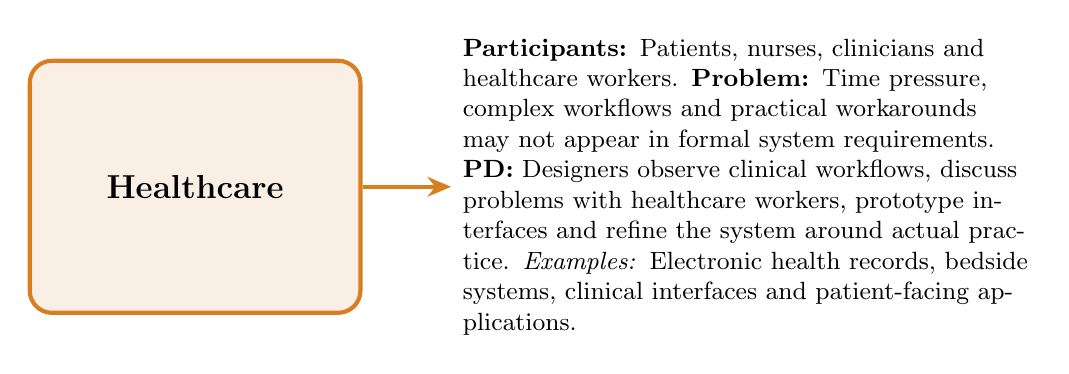
\begin{tikzpicture}[>=Stealth]
\node[
rounded corners=8pt,
draw=myorange,
fill=myorange!12,
line width=1.5pt,
minimum width=4.2cm,
minimum height=3.2cm,
text width=3.6cm,
align=center,
font=\bfseries\large,
inner sep=8pt
] (health) {\textbf{Healthcare}};

\node[
text width=7.2cm,
align=left,
font=\small,
inner sep=4pt
] (healthtext) at (7,0) {
\textbf{Participants:} Patients, nurses, clinicians and healthcare
workers. 
\textbf{Problem:} Time pressure, complex workflows and practical
workarounds may not appear in formal system requirements. 
\textbf{PD:} Designers observe clinical workflows, discuss problems
with healthcare workers, prototype interfaces and refine the system
around actual practice. 
\textit{Examples:} Electronic health records, bedside systems,
clinical interfaces and patient-facing applications.
};

\draw[-{Stealth[length=3mm,width=2.5mm]},
line width=1.4pt,myorange]
(health.east) -- (healthtext.west);
\end{tikzpicture}
\end{center}

\vspace{0.5cm}

% ==========================================================
% 2. EDUCATION
% ==========================================================
\begin{center}
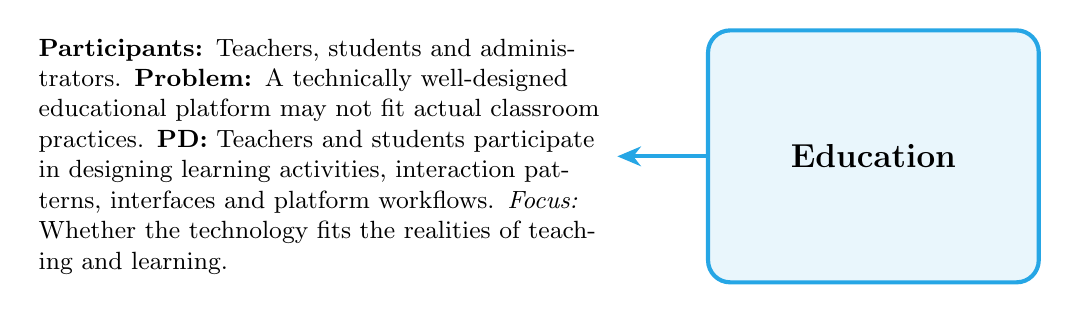
\begin{tikzpicture}[>=Stealth]
\node[
rounded corners=8pt,
draw=myblue,
fill=myblue!10,
line width=1.5pt,
minimum width=4.2cm,
minimum height=3.2cm,
text width=3.6cm,
align=center,
font=\bfseries\large,
inner sep=8pt
] (education) at (7,0) {\textbf{Education}};

\node[
text width=7.2cm,
align=left,
font=\small,
inner sep=4pt
] (educationtext) at (0,0) {
\textbf{Participants:} Teachers, students and administrators. 
\textbf{Problem:} A technically well-designed educational platform
may not fit actual classroom practices. 
\textbf{PD:} Teachers and students participate in designing learning
activities, interaction patterns, interfaces and platform workflows. 
\textit{Focus:} Whether the technology fits the realities of teaching
and learning.
};

\draw[-{Stealth[length=3mm,width=2.5mm]},
line width=1.4pt,myblue]
(education.west) -- (educationtext.east);
\end{tikzpicture}
\end{center}

\vspace{0.5cm}

% ==========================================================
% 3. GOVERNMENT
% ==========================================================
\begin{center}
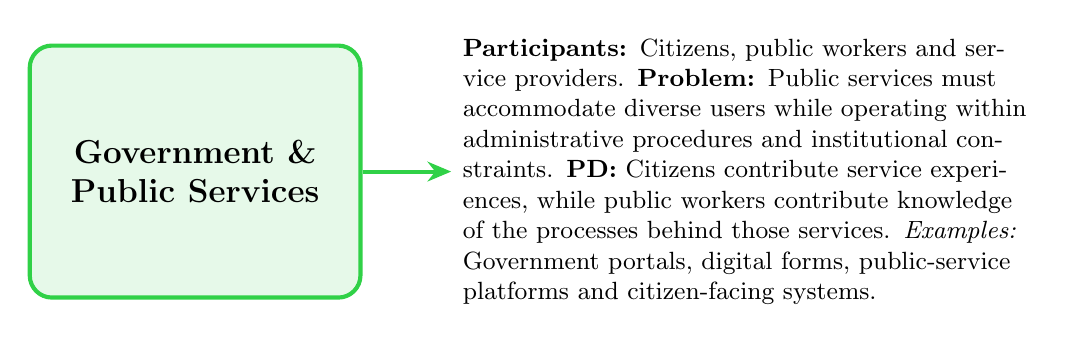
\begin{tikzpicture}[>=Stealth]
\node[
rounded corners=8pt,
draw=mygreen,
fill=mygreen!12,
line width=1.5pt,
minimum width=4.2cm,
minimum height=3.2cm,
text width=3.6cm,
align=center,
font=\bfseries\large,
inner sep=8pt
] (government) {\textbf{Government \& Public Services}};

\node[
text width=7.2cm,
align=left,
font=\small,
inner sep=4pt
] (governmenttext) at (7,0) {
\textbf{Participants:} Citizens, public workers and service providers. 
\textbf{Problem:} Public services must accommodate diverse users while
operating within administrative procedures and institutional
constraints. 
\textbf{PD:} Citizens contribute service experiences, while public
workers contribute knowledge of the processes behind those services. 
\textit{Examples:} Government portals, digital forms, public-service
platforms and citizen-facing systems.
};

\draw[-{Stealth[length=3mm,width=2.5mm]},
line width=1.4pt,mygreen]
(government.east) -- (governmenttext.west);
\end{tikzpicture}
\end{center}

\vspace{0.5cm}

% ==========================================================
% 4. WORKPLACE
% ==========================================================
\begin{center}
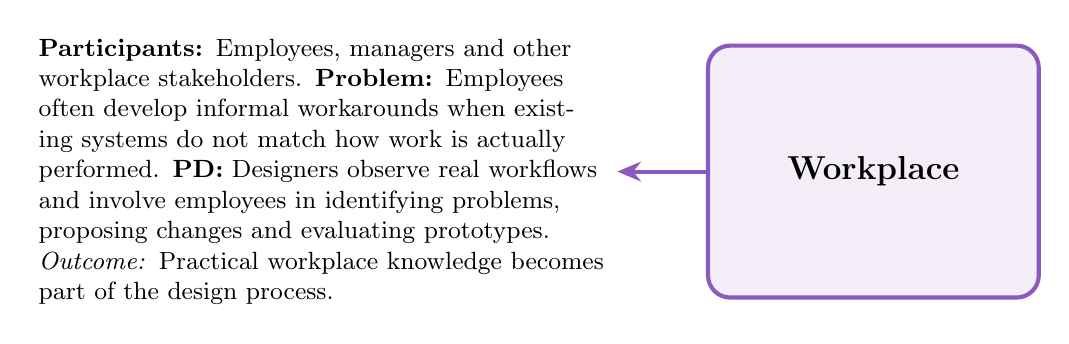
\begin{tikzpicture}[>=Stealth]
\node[
rounded corners=8pt,
draw=mypurple,
fill=mypurple!10,
line width=1.5pt,
minimum width=4.2cm,
minimum height=3.2cm,
text width=3.6cm,
align=center,
font=\bfseries\large,
inner sep=8pt
] (workplace) at (7,0) {\textbf{Workplace}};

\node[
text width=7.2cm,
align=left,
font=\small,
inner sep=4pt
] (workplacetext) at (0,0) {
\textbf{Participants:} Employees, managers and other workplace
stakeholders. 
\textbf{Problem:} Employees often develop informal workarounds when
existing systems do not match how work is actually performed. 
\textbf{PD:} Designers observe real workflows and involve employees in
identifying problems, proposing changes and evaluating prototypes. 
\textit{Outcome:} Practical workplace knowledge becomes part of the
design process.
};

\draw[-{Stealth[length=3mm,width=2.5mm]},
line width=1.4pt,mypurple]
(workplace.west) -- (workplacetext.east);
\end{tikzpicture}
\end{center}

\vspace{0.5cm}

% ==========================================================
% 5. ASSISTIVE TECHNOLOGY
% ==========================================================
\begin{center}
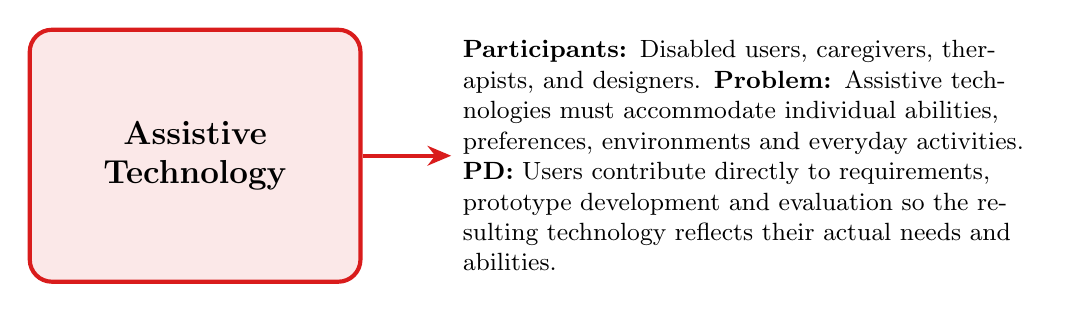
\begin{tikzpicture}[>=Stealth]
\node[
rounded corners=8pt,
draw=myred,
fill=myred!10,
line width=1.5pt,
minimum width=4.2cm,
minimum height=3.2cm,
text width=3.6cm,
align=center,
font=\bfseries\large,
inner sep=8pt
] (assistive) {\textbf{Assistive Technology}};

\node[
text width=7.2cm,
align=left,
font=\small,
inner sep=4pt
] (assistivetext) at (7,0) {
\textbf{Participants:} Disabled users, caregivers, therapists, and
designers. 
\textbf{Problem:} Assistive technologies must accommodate individual
abilities, preferences, environments and everyday activities. 
\textbf{PD:} Users contribute directly to requirements, prototype
development and evaluation so the resulting technology reflects
their actual needs and abilities.
};

\draw[-{Stealth[length=3mm,width=2.5mm]},
line width=1.4pt,myred]
(assistive.east) -- (assistivetext.west);
\end{tikzpicture}
\end{center}

\vspace{0.5cm}

% ==========================================================
% 6. TECHNOLOGY & PRODUCT DEVELOPMENT
% ==========================================================
\begin{center}
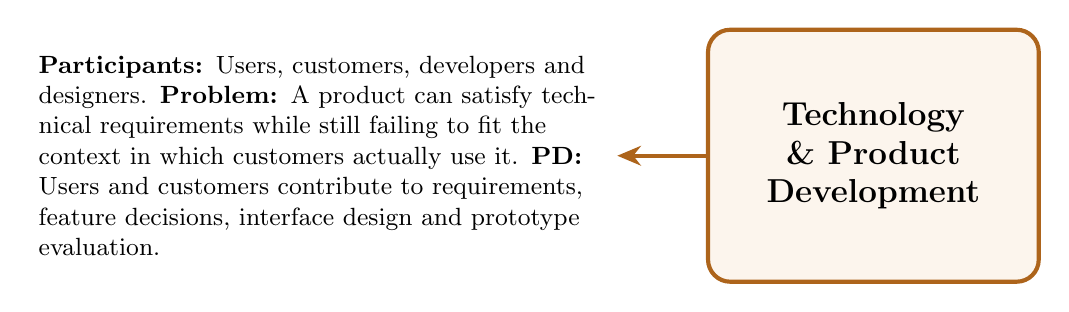
\begin{tikzpicture}[>=Stealth]
\node[
rounded corners=8pt,
draw=myorange!80!black,
fill=myorange!8,
line width=1.5pt,
minimum width=4.2cm,
minimum height=3.2cm,
text width=3.6cm,
align=center,
font=\bfseries\large,
inner sep=8pt
] (technology) at (7,0)
{\textbf{Technology \& Product Development}};

\node[
text width=7.2cm,
align=left,
font=\small,
inner sep=4pt
] (technologytext) at (0,0) {
\textbf{Participants:} Users, customers, developers and designers. 
\textbf{Problem:} A product can satisfy technical requirements while
still failing to fit the context in which customers actually use it. 
\textbf{PD:} Users and customers contribute to requirements, feature
decisions, interface design and prototype evaluation.
};

\draw[-{Stealth[length=3mm,width=2.5mm]},
line width=1.4pt,myorange!80!black]
(technology.west) -- (technologytext.east);
\end{tikzpicture}
\end{center}

Across these domains, the context differs, but the underlying principle is
the same: the people who live with a system should have an opportunity to
influence its design.



%==========================================================
\section{Benefits of Participatory Design}
\label{sec:benefits}
%==========================================================

We can understand the value of Participatory Design through three connected
layers: \textbf{people}, \textbf{insight} and \textbf{outcome}. Participation
gives stakeholders a voice, their involvement reveals contextual knowledge,
and that knowledge can influence the resulting design.


\subsection{Voice and Ownership}

Participatory Design gives people affected by a system an opportunity to
express their needs and influence design decisions. This can create a
stronger sense of ownership because participants can see their contributions
reflected in the resulting system.


\subsection{Context and Domain Knowledge}

Users possess practical knowledge about their everyday work, including
workarounds, exceptions, constraints and informal practices. Such knowledge
may not appear in formal requirements. Direct participation allows designers
to discover this context while the team is still developing the design.


\subsection{Improved Usability and Feasibility}

Continuous involvement allows users to identify problems in interfaces and
workflows before deployment. Participants can also identify whether a
proposed solution is realistic within existing practices, resources and
organizational constraints.


\subsection{Diverse Perspectives and Innovation}

Different stakeholders may experience the same system in very different
ways. Bringing these perspectives together can reveal problems and possible
solutions that would otherwise remain hidden from the design team.


\subsection{The Flow of Benefits}

These benefits form a flow from people to insight to outcome, which
Figure~\ref{fig:peopleinsightoutcome} shows. People contribute \textbf{voice and ownership}; participation produces
\textbf{context and knowledge}; and these insights can contribute to
\textbf{usability, feasibility and innovation}.

\begin{figure}[H]
\centering
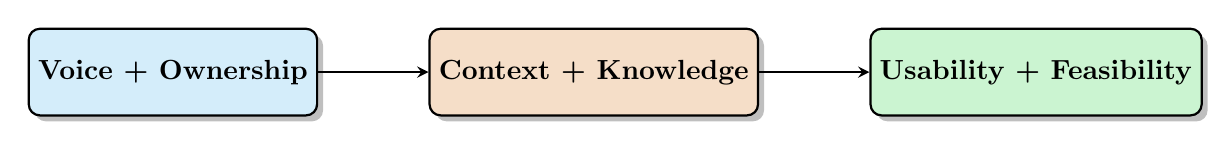
\begin{tikzpicture}[
    node distance=1.4cm,
    box/.style={
        rectangle,
        rounded corners,
        minimum width=3.2cm,
        minimum height=1.1cm,
        text centered,
        draw=black,
        thick,
        drop shadow
    }
]
    \node[box, fill=myblue!20] (people)
        {\textbf{Voice + Ownership}};

    \node[box, fill=myorange!25, right=of people]
        (insight)
        {\textbf{Context + Knowledge}};

    \node[box, fill=mygreen!25, right=of insight]
        (outcome)
        {\textbf{Usability + Feasibility}};

    \draw[arrow] (people) -- (insight);
    \draw[arrow] (insight) -- (outcome);
\end{tikzpicture}
\caption{The people--insight--outcome relationship in Participatory Design}
\label{fig:peopleinsightoutcome}
\end{figure}

%==========================================================
\section{Challenges of Participatory Design}
\label{sec:challenges}
%==========================================================

Participatory Design creates value by involving multiple stakeholders, but
participation also introduces practical tensions. Different stakeholders may
want different outcomes, participants may have limited time, expectations
may become difficult to manage, and some projects involve sensitive
information. The challenge is therefore not simply to increase participation,
but to structure it effectively.


\subsection{Conflicting Needs}

Different stakeholders may prioritize different outcomes. For example, in a
healthcare system, nurses may prioritize speed, IT staff may prioritize
security and compliance, while management may prioritize cost.

Participatory Design does not guarantee agreement. Instead, it provides a
setting in which stakeholders can make disagreement visible and discuss
trade-offs openly.

\textbf{Response:} Make competing requirements explicit and negotiate
trade-offs among stakeholders.


\subsection{Time and Logistics}

Frontline users are often busy, and bringing people from different roles
together can make workshops difficult to organize. Repeated participation
may also increase the time required for a project.

\textbf{Response:} Short micro-sessions, targeted participant groups and
asynchronous activities can reduce the burden while preserving meaningful
participation.


\subsection{Trust and Expectations}

Participants may question whether designers will actually listen to their
contributions. At the same time, participants may expect the team to implement
every suggestion, even when technical, financial or organizational
constraints make this impossible.

\textbf{Response:} Designers should be transparent about constraints and
show participants how their feedback influenced subsequent design decisions.


\subsection{Participation and Privacy}

Some Participatory Design projects involve sensitive information. Healthcare
projects may involve medical records, government projects may involve
confidential citizen information, and enterprise projects may contain
proprietary information.

Therefore, meaningful participation does not require every participant to
have access to every piece of information.


\subsubsection{The Need-to-Know Boundary}

A useful principle is that participation can be broad in purpose while access
remains narrow in scope.

A team can protect sensitive information in four ways, which
Table~\ref{tab:privacy} summarizes:

\begin{itemize}
    \item \textbf{Synthetic data} instead of real personal records;
    \item \textbf{Task abstraction} so that participants can discuss workflows
    without exposing sensitive details;
    \item \textbf{Role-based access} so participants see only information
    necessary for their contribution;
    \item \textbf{Confidentiality measures} where appropriate.
\end{itemize}

\begin{table}[H]
\centering
\begin{tabularx}{\textwidth}{@{}l X@{}}
\toprule
\rowcolor{myblue!20}
\textbf{Protection} & \textbf{Purpose} \\
\midrule
Synthetic data & Allows participation without exposing real sensitive data \\
Task abstraction & Separates design discussion from private details \\
Role-based access & Limits information according to participant needs \\
Confidentiality & Establishes responsibilities for sensitive information \\
\bottomrule
\end{tabularx}
\caption{Approaches for balancing participation and privacy}
\label{tab:privacy}
\end{table}


\subsection{Managing the Challenges}

The four challenges above do not mean that teams should reduce participation.
Instead, they show why teams must structure participation deliberately.
Table~\ref{tab:challenge_response} summarizes each challenge and the
corresponding response.

\begin{table}[H]
\centering
\begin{tabularx}{\textwidth}{@{}l X X@{}}
\toprule
\rowcolor{myblue!20}
\textbf{Challenge} & \textbf{Problem} & \textbf{Response} \\
\midrule
Conflict & Stakeholders have different priorities &
Open negotiation and explicit trade-offs \\

Time & Users have limited availability &
Short and targeted sessions \\

Trust & Participants may doubt their influence &
Transparency and visible impact \\

Privacy & Participation may involve sensitive information &
Need-to-know access and protected data \\
\bottomrule
\end{tabularx}
\caption{Major challenges and corresponding responses}
\label{tab:challenge_response}
\end{table}

%==========================================================
\section{Conclusion}
\label{sec:conclusion}
%==========================================================

Participatory Design represents a shift in the way teams conceive and
develop systems. Instead of treating users as people for whom designers build
a system, PD involves the people affected by the system in shaping it.
Figure~\ref{fig:conclusionflow} restates this idea as a flow from people to
insight to outcome.

\begin{figure}[H]
\centering
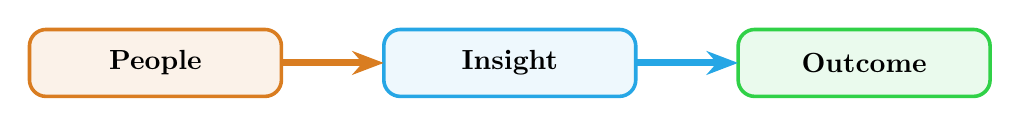
\begin{tikzpicture}[>=Stealth]
\node[
draw=myorange,
fill=myorange!10,
line width=1.3pt,
rounded corners=6pt,
minimum width=3.2cm,
minimum height=0.85cm,
align=center
] {\textbf{People}};

\node[
draw=myblue,
fill=myblue!8,
line width=1.3pt,
rounded corners=6pt,
minimum width=3.2cm,
minimum height=0.85cm,
xshift=4.5cm,
align=center
] {\textbf{Insight}};

\node[
draw=mygreen,
fill=mygreen!10,
line width=1.3pt,
rounded corners=6pt,
minimum width=3.2cm,
minimum height=0.85cm,
xshift=9cm,
align=center
] {\textbf{Outcome}};

\draw[-{Stealth[length=4mm,width=3mm]}, line width=2.5pt, myorange]
(1.6,0) -- (2.9,0);

\draw[-{Stealth[length=4mm,width=3mm]}, line width=2.5pt, myblue]
(6.1,0) -- (7.4,0);
\end{tikzpicture}
\caption{People, insight and outcome in Participatory Design}
\label{fig:conclusionflow}
\end{figure}

Its applications demonstrate that this principle is not limited to a single
industry. Healthcare, education, government, workplaces, assistive
technology and product development all involve situations where users
possess important knowledge about the context in which a system operates.

Participation creates value through the connection between people, insight
and outcome. Participants contribute their perspectives, which can reveal
contextual knowledge, workarounds and diverse needs, ultimately contributing
to more usable and feasible designs.

However, participation is not automatically successful. Conflicting needs,
limited time, trust and privacy can create significant difficulties.
Effective Participatory Design therefore requires carefully structured
participation, transparent communication and appropriate boundaries around
sensitive information.



\subsection{The Central Takeaway}

We can summarize the central idea of Participatory Design as a change in
design perspective, which Figure~\ref{fig:forwith} shows.

\begin{figure}[H]
\centering
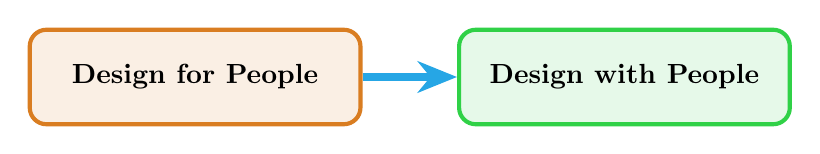
\begin{tikzpicture}[>=Stealth, node distance=1.2cm]
\node[
draw=myorange,
fill=myorange!12,
line width=1.5pt,
rounded corners=6pt,
minimum width=4.2cm,
minimum height=1.2cm,
align=center
] (for) {\textbf{Design for People}};

\node[
    draw=mygreen,
    fill=mygreen!12,
    line width=1.5pt,
    rounded corners=6pt,
    minimum width=4.2cm,
    minimum height=1.2cm,
    align=center,
    right=of for
] (with) {\textbf{Design with People}};

\draw[
    -{Stealth[length=5mm,width=4mm]},
    line width=3pt,
    myblue
] (for) -- (with);

\end{tikzpicture}
\caption{The shift from designing for people to designing with people}
\label{fig:forwith}
\end{figure}

Participatory Design therefore matters not simply because designers ask users
for their opinions, but because it gives the people affected by a system a
meaningful opportunity to help shape it.



\newpage
\addcontentsline{toc}{section}{References}
\bibliography{references}

\end{document}